\chapter{Task \# 44 - Social Connectedness Index  from Facebook}

\resp{Jacopo Carotenuto}
\section{Introduction}
In this task the goal was to extract a network for each country present in the Facebook Scaled Social Connectedness Index data \cite{FacebookSocialConnectednessIndexData}.
The data was collected by Facebook and it is based on the number of friendships between people in different countries.
From the documentation:
\begin{quote}
The Social Connectedness Index uses an anonymized snapshot of active Facebook users and their friendship networks to measure the intensity of social connectedness between locations. Users are assigned to locations based on their information and activity on Facebook, including the stated city on their Facebook profile, and device and connection information.
\end{quote}

\section{Network Extraction}
\subsection{Raw Data}
The goal was to build two files:
\begin{enumerate}
    \item \texttt{node\_list.csv}: a file containing the node ID, longitude, latitude and label for each node.
    \item \texttt{edge\_list.csv}: a file containing the source node ID, target node ID, weight (SCI), country and country ISO code for each edge.
\end{enumerate}
As the goal was to build a network for each country, edges between different countries were not considered.
The data provided was in a ".tsv" file with the following columns: "\texttt{user\_loc}", "\texttt{fr\_loc}" and "\texttt{scaled\_sci}" representing the User Location, Friend Location and Scaled Social Connectedness Index respectively.
As written in the documentation, the SSCI was built to be between $1$ and $10^9$.
All data manipulation and analysis were done in Julia\cite{julia}.

\subsection{Edge List}
The first step was to extract all the unique locations present in the data and assign a unique ID to each of them. As the location were divided in different types of denominations (GADM\cite{GADM}, NUTS\cite{NUTS} and US Counties) the file "\texttt{gadm1\_nuts3\_counties\_levels.csv}" was used to determine the type of denomination for each location.
Then each location was assigned the ISO3 code of the country it belonged to using the "Countries" package in Julia\cite{countries_package}.
To each entry of the original file (so to each edge) the User ISO3 code and the Friend ISO3 code were added and all the edges between different countries were removed.
The final edge list was saved in a ".csv" file, saving only the source node ID, target node ID, weight, country and country ISO code.
For completeness, the edge list present all the (symmetric) edges present in the source file.

\subsection{Node List}
The node list was more of a challenge as the longitude and latitude of each location were not provided.
To assign to each location its coordinates, the geospatial data for each subdivision was found:
\begin{itemize}
    \item For the GADM subdivisions, the data was found in the GADM website\cite{GADM} (Version 2.8, world data).
    \item For the NUTS subdivisions, the data was found in the Eurostat website\cite{NUTS} (Year 2016, EPSG 4326).
    \item For the US counties, the data was found in the Public Data website\cite{USCounties} (Year 2018).
\end{itemize}
The provided data was in the form of a ".shp" or ".geojson" files, so for the coordinates extraction the "GeoStats.jl" package was used\cite{geostats_package}. For all the administrative subdivision a polygon was provided, so the centroid of each polygon was used as the coordinates for the location. As the provided Facebook data contained different levels of administrative subdivisions, each level was analyzed separately.
Then, as the Facebook area code used was different from all the other denominations, the area codes of each location were transformed in the Facebook format.
Then, for each unique node we associated the coordinates and the label (also found in the official data).
The final node list was saved in a ".csv" file, saving the node ID, longitude, latitude and label.

\section{Network Comparison}
The resulting countries SCI-weighted undirected network were all analyzed using Julia and some important network properties were extracted. Some of them are contained in the following plots.

\begin{figure}[H]
    \centering
    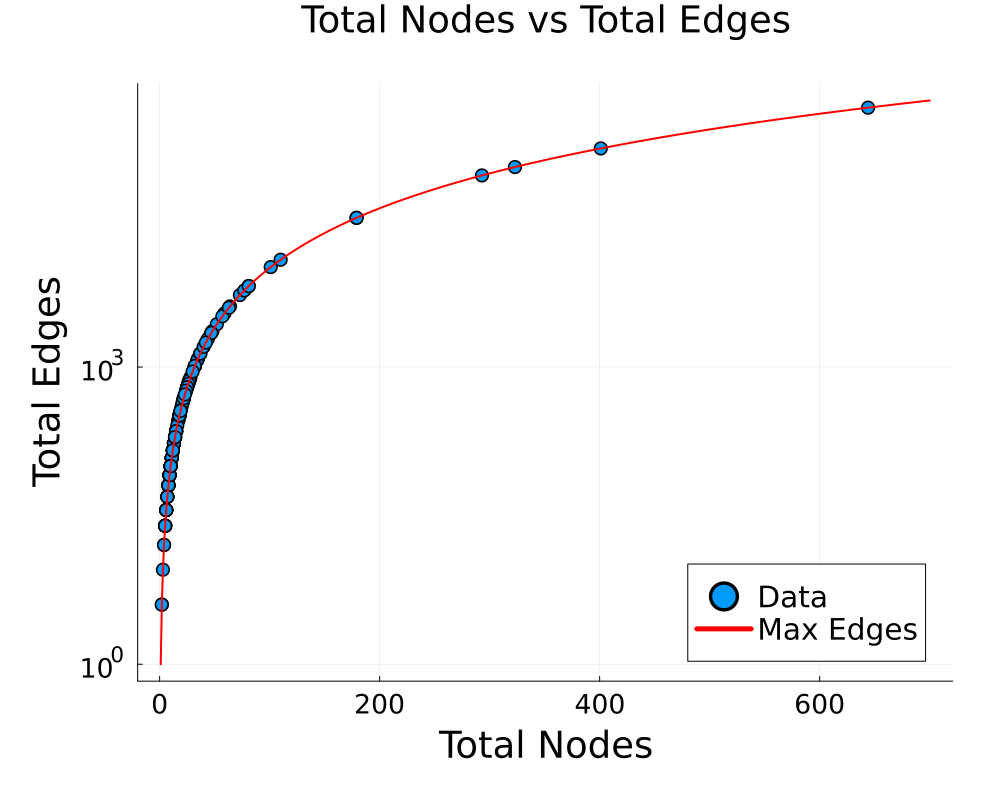
\includegraphics[width=0.6\textwidth]{images/task44/TotalNodesVsTotalEdges.png}
    \caption{}
    \label{fig:TotalNodesVsTotalEdges}
\end{figure}

From plot~\ref{fig:TotalNodesVsTotalEdges} we can see that the number of edges is proportional to the number of nodes (it's exactly the maximum number of undirected connections, allowing for self-loops), as expected as all the networks are complete networks: every location has at least some people connected to every other location in the same country.

 
\begin{figure}[H]
    \centering
    \begin{minipage}{0.5\textwidth}
        \centering
        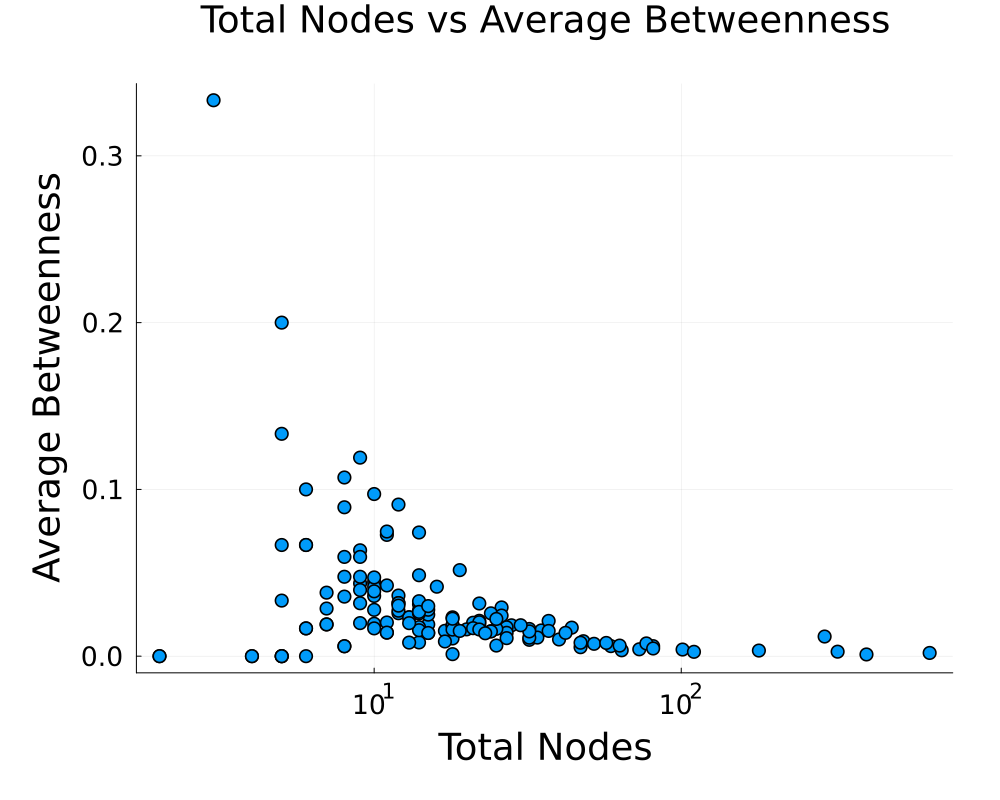
\includegraphics[width=1\linewidth]{images/task44/TotalNodesVsAverageBetweenness.png}
    \end{minipage}%
    \begin{minipage}{0.5\textwidth}
        \centering
        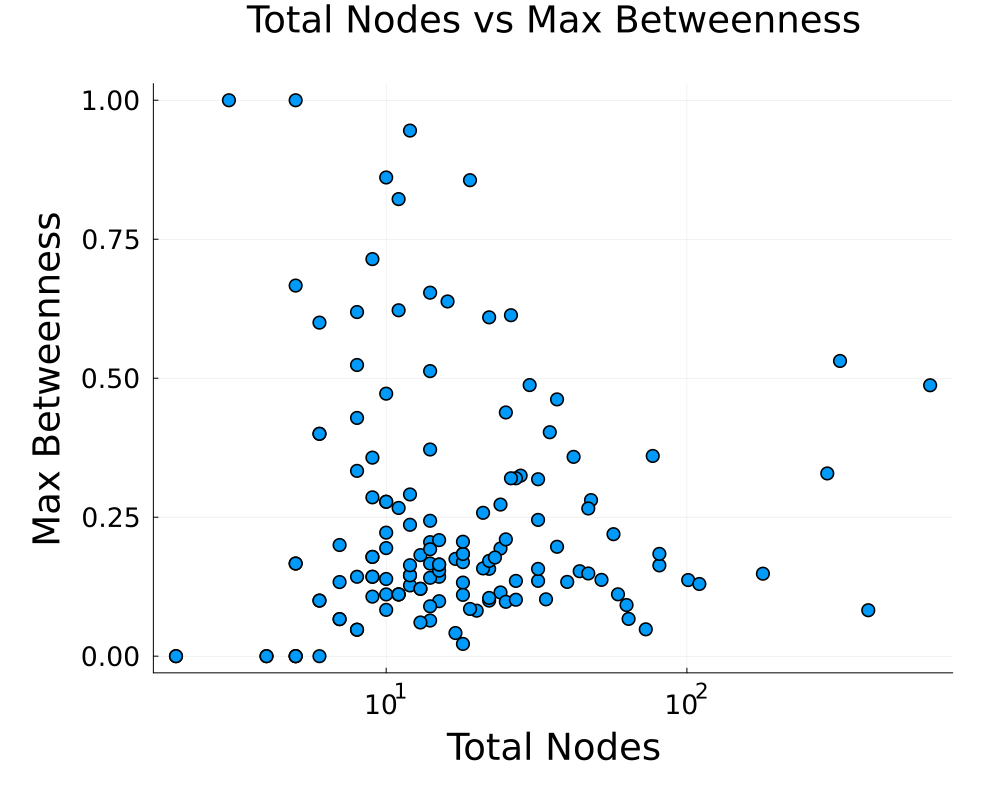
\includegraphics[width=1\linewidth]{images/task44/TotalNodesVsMaxBetweenness.png}
    \end{minipage}
    \caption{}
    \label{fig:TotalNodesVsMaxBetweenness}
    \label{fig:TotalNodesVsAverageBetweenness}
\end{figure}


From plot~\ref{fig:TotalNodesVsAverageBetweenness} we can see that the average betweenness is inversely proportional to the number of nodes in a exponential way but the maximum betweenness is less correlated with the number of nodes.

\begin{figure}[H]
    \centering
    \begin{minipage}{0.48\textwidth}
        \centering
        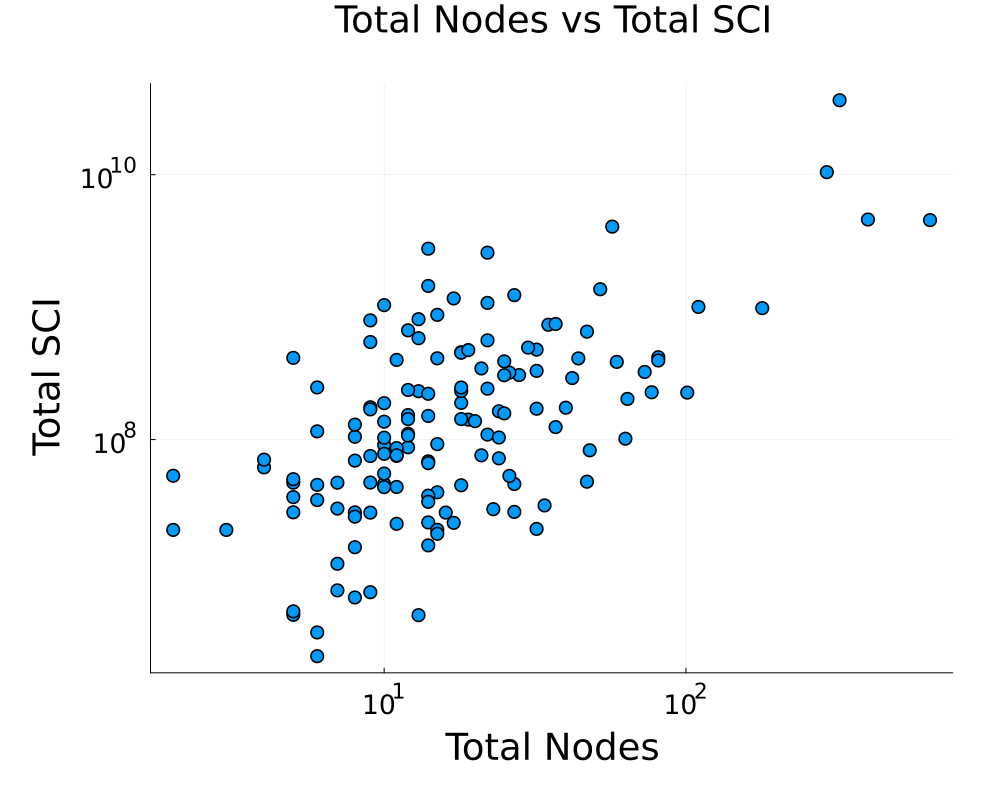
\includegraphics[width=1\textwidth]{images/task44/TotalNodesVsTotalSCI.png}
    \end{minipage}
    \begin{minipage}{0.5\textwidth}
        \centering
        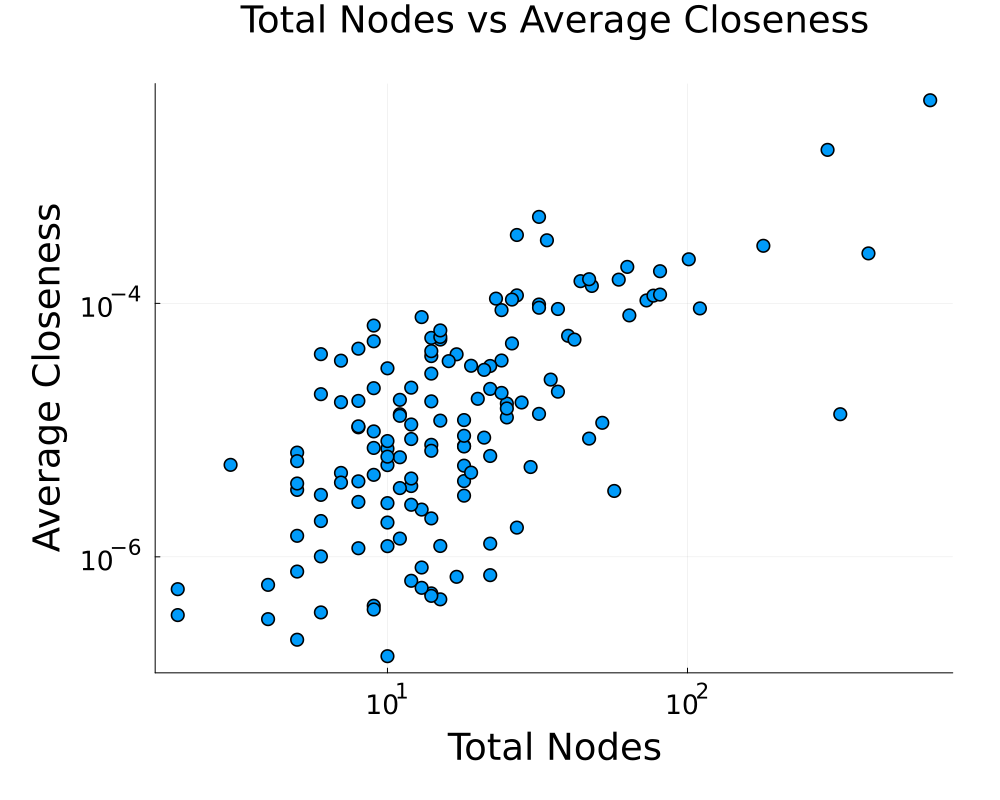
\includegraphics[width=1\textwidth]{images/task44/TotalNodesVsAverageCloseness.png}
    \end{minipage}
    \caption{}
    \label{fig:TotalNodesVsAverageCloseness}
    \label{fig:TotalNodesVsTotalSCI}
\end{figure}

From plot~\ref{fig:TotalNodesVsAverageCloseness} it can be seen that the number of nodes is proportional to both the average closeness and the total SCI.

\newpage